%\documentclass{emulateapj}
\documentclass[letterpaper,12pt,preprint]{aastex}

% packages
\usepackage{amssymb,amsmath,amsbsy}
\usepackage{bbold}
\usepackage{arydshln}
\usepackage{algpseudocode}
\renewcommand\algorithmicthen{}
\renewcommand\algorithmicdo{}
\usepackage{mathrsfs}
\usepackage{subfigure}
\usepackage[backref,breaklinks,colorlinks,citecolor=blue]{hyperref}

% commands
\newcommand{\given}{\,|\,}
\newcommand{\dd}{\mathrm{d}}
\newcommand{\transpose}[1]{{#1}^{\mathsf{T}}}
\newcommand{\inverse}[1]{{#1}^{-1}}
\newcommand{\msun}{\mathrm{M}_\odot}
\newcommand{\bs}[1]{\boldsymbol{#1}}
\newcommand{\ident}{\mathbb{1}}
\newcommand{\inttime}{t_{\rm int}}
\newcommand{\fdrate}{\mathcal{R}_\Omega}

\newcommand{\act}{J}
%\newcommand{\jac}{\bs{\rm J}}
%\newcommand{\jac}{\bs{G}}
\newcommand{\jac}{\mathscr{J}}

\begin{document}

%TODO:
%The classical way to detect chaotic motion is
%the computation of the Lyapunov exponents. We
%claim that for weakly chaotic solutions, the frequency
%analysis gives information more rapidly
%and more precisely. The reason is that the frequency
%analysis is an instantaneous observation
%of the fundamental frequencies which are essential
%parameters of the dynamical system, while
%the usual computation of Lyapunov exponents
%acts like a mean and needs a very long time span
%to provide reliable results (for references and
%discussion on Lyapunov exponents, see refs. [3,
%12]. 

% Highlight that stochastic tubes have not been studied much...

\title{Tidal streams in triaxial systems}
\author{Adrian M. Price-Whelan\altaffilmark{\colum,\adrn},
	    Kathryn V. Johnston\altaffilmark{\colum},
	    Monica Valluri\altaffilmark{\mich}}
\date{\centering \today}

% Affiliations
\newcommand{\colum}{1}
\newcommand{\adrn}{2}
\newcommand{\mich}{3}
\altaffiltext{\colum}{Department of Astronomy, 
		              Columbia University, 
		              550 W 120th St., 
		              New York, NY 10027, USA}
\altaffiltext{\adrn}{To whom correspondence should be addressed: adrn@astro.columbia.edu}
\altaffiltext{\mich}{Department of Astronomy, 
			   University of Michigan,
			   Ann Arbor, MI 48109, USA}

\begin{abstract}

Tidal streams form from the steady disruption of stellar systems
orbiting within the gravitational field of some parent galaxy. Many
streams and debris structures have been discovered in the halo of the
Milky Way and have been used to model the potential of the Galaxy. 
However, few of these models have yet explored the properties of
tidal debris in triaxial potentials.
The existence of a variety of orbits, resonances, and chaotic regions in such potentials 
suggest that the morphologies and dispersal timescales of
debris could differ significantly from the simpler spherical and oblate cases.
In this work we use a series of N-body simulations of stellar systems over a range 
of masses of disruption in triaxial potentials to understand the influence of the nature 
and types of orbits on debris morphologies.
Our results suggest that the mere existence of the multitude of thin streams
already known to orbit the Milky Way provides significant constraints on the
classes of triaxial potentials that provide a good representation for its dark matter halo.

\end{abstract}

\keywords{
}

%\begin{figure*}[!h]
%\begin{center}
%\includegraphics[width=\textwidth]{PATH}
%\caption{ CAPTION }\label{fig:FIGNAME}
%\end{center}
%\end{figure*}

\section{Introduction}\label{sec:introduction}

On the largest scales ($\gtrsim$30~kpc for a Milky-Way-like galaxy) in the halos of galaxies, gravitational potentials are thought to be triaxial. Despite suggestive evidence from a range of complimentary techniques, this fundamental prediction from $\Lambda$CDM cosmology has not been conclusively verified by observations. Around other galaxies, it is generally hard to measure the 3D mass profile because they are seen in projection. From the Earth's position within the Milky Way, our view of our own halo and proximity gives us a unique chance to directly measure the 6D positions of stars and model the shape of the mass distribution at large radii. Unfortunately, the Milky Way halo has a low density of visible tracers, but luckily many of the halo stars are likely associated with debris stripped from in-falling satellite galaxies.

As a satellite galaxy or globular cluster orbits within some larger system, mass is eroded due to the tidal forces of the host galaxy potential. If the orbit of such an object is regular, only mildly eccentric, and stays far from sharp density features (e.g., the disk), the disruption is a steady process and the mass is slowly stretched into long streams of matter. The phase-space density and therefore the observable properties of these tidal streams are sensitive to the internal progenitor properties, orbit of the progenitor, and underlying mass distribution of the host galaxy. The morphological evolution of the debris depends on the spread of orbital properties (e.g., actions or frequencies) of the debris and the orbit of the progenitor system, both of which are also set by the shape and radial profile of the gravitational potential of the host galaxy. In the halo of the Milky Way, tidal streams of stars are found over a large range of distances ($\sim$10-100~kpc). By simultaneously modeling the observed phase-space density of stream stars along with the potential, it is hoped that we may infer the dark matter distribution of the Milky Way on these scales.

Tidal streams are generally modeled as 1D structures formed on regular orbits with simple internal progenitor dynamics and density evolution. Methods span a range of complexity from orbit-fitting, to \emph{Streakline} or particle-spray models, to action-space density modeling, to direct $N$-body simulations. All methods have been tested in some way on simulated observations of data and authors have mainly demonstrated their ability to recover parameters of analytic, static potential forms. Many of the methods have been shown to work in axisymmetric or otherwise simple potentials but claim to extend to more complex, generalized potentials (e.g., triaxial or multi-component potentials). 

\citet{pearson15} tried to reproduce observations of the stellar stream density from the globular cluster Palomar 5 in a single oblate and single triaxial potential using \emph{Streakline} models \citep{kuepper12}. They use the observed SDSS number density of stars and a limited number of radial velocities measured for stream members to fit model streams to the data. In the oblate potential (a three-component, bulge, disk, and spherical halo potential), a thin model stream is easily found that reproduces the observed stellar density morphology of the stream. In the triaxial potential (the potential from \cite{law10}, a three component, bulge, disk, and triaxial halo fit to Sagitarrius stream data), the model streams generically form large, two-dimensional ``fans'' of debris near the ends, and there are no physically reasonable progenitor orbits that reproduce the observed thinness of the stream given the observational constraints of the present-day position and velocity of the cluster. This result suggests that the shape of the host galaxy potential directly influences the morphology of the resulting debris. In order to extend tidal stream models to more generic potentials, it is important to understand why this stream-fanning occurs and whether this and other strange debris morphologies are generic to more complex potentials. This also has implications for modeling the accretion histories of galaxies. Debris morphology is often separated into two classes --- streams (usually from high angular momentum progenitor orbits) and shells (from radially plunging orbits) --- but in practice the distinction may not be as clear due to other mixing effects.

The obvious difference between the two potentials considered by \citet{pearson15} is the extra symmetry of the oblate potential. For an integrable Hamiltonian, $H$, with $N$ degrees of freedom (dof), the equations of motion are most simply expressed in angle-action coordinates \cite[e.g.,][]{goldstein80}. In these coordinates, the actions, $J_n$, are integrals of the motion, and the conjugate angle variables, $\theta_n$, increase linearly with time
\begin{align}
	\dot{\act}_n &= -\frac{\partial H}{\partial \theta_n} = 0\\
	\act_n &= {\rm const.}\\
	\dot{\theta}_n &= \frac{\partial H}{\partial \act_n} = \Omega_n(\act_1,\act_2,...,\act_n)\label{eq:aafreq}\\
	\theta_n(t) &= \Omega_n t + \theta_n(0)
\end{align}
where $i=1,2,...N$, and $\Omega_n$ are the fundamental frequencies of the orbit. The topology of angle-action space is equivalent to that of the surface of an $N$-dimensional torus, and thus orbits are often referred to in terms of \emph{orbital tori}: each set of actions, $(\act_1,\act_2,...\act_N)$, uniquely ``label'' the torus associated with a given orbit and the angles specify the location on the surface of the $N$-torus. If a global transformation to angle-action coordinates exists, the potential is said to be \emph{integrable}.

If galactic halos are triaxial, galactic gravitational potentials will almost certainly not be globally integrable. If a triaxial (three dof) potential is close to integrable such that the Hamiltonian can be written in terms of a small perturbation, $\epsilon$, away from some integrable Hamiltonian, $H_0$,
\begin{equation}
	H(\bs{\theta}, \bs{\act}) = H_0(\bs{\act}) + \epsilon H_1(\bs{\theta}, \bs{\act})
\end{equation}
then a large number of regular orbits will survive the perturbation (by way of the KAM theorem)\footnote{3-vectors are represented with bold symbols, e.g., $\bs{J}=(J_1,J_2,J_3)$.}. The tori that survive will in general be separated by regions of irregular or chaotic motion, and thus any transformations to angle-action coordinates can only be defined locally. Analytic transformations to angle-action coordinates are only known for a handful of simple, integrable potentials. Much effort has gone in to developing general methods for transforming either from position-velocity to angle-action coordinates, $(\bs{x},\bs{v})\rightarrow(\bs{\theta},\bs{J})$ \citep{many}, or vice-versa, $(\bs{\theta},\bs{J})\rightarrow(\bs{x},\bs{v})$ \citep{many}.

The types of motion generic to triaxial systems can be split into several sub-categories (summarized in Figure~\ref{fig:orbit-tree}). Regular motion can be classified by the number of resonance relations obeyed \citep[e.g.,][]{lichtenberg83, valluri98}: \emph{conditionally periodic} orbits obey no resonance relations, \emph{uni-resonant} orbits obey a single relation of the form $\bs{m}\cdot\bs{\Omega}=0$, and \emph{bi-resonant} orbits obey two resonance relations, $\bs{m}\cdot\bs{\Omega}=0$ and $\bs{n}\cdot\bs{\Omega}=0$, where $\bs{m}$ and $\bs{n}$ are integer vectors.

\begin{figure*}[!h]
\begin{center}
\includegraphics[width=0.5\textwidth]{figures/orbit-tree.pdf}
\caption{} \label{fig:orbit-tree}
\end{center}
\end{figure*}

Resonant orbits are rare \citep{merritt99} but dynamically important in systems with several degrees of freedom as they determine the structure of orbit-space. Stable, resonant orbits generate families of orbits that may behave or appear similarly, whereas unstable resonances are typically associated with regions of chaos. Not all orbits can be trivially associated with resonances due to the infinitely complex, hierarchical structure of resonances (though the importance or ``size'' of a resonance falls off inversely with the norm of its integer vector, $|\bs{m}|^{-\alpha}$, with $\alpha > 0$). In autonomous, two dof systems, stochastic regions are generally surrounded and separated by regular motion, thus chaotic orbits are confined. In three or more dof the chaotic regions will connect and overlap. This is the origin of Arnold diffusion \citep{arnold64}, which allows chaotic orbits to radically change shape by traversing the web of unstable resonances and are only strictly bounded to their own energy hypersurface. This phenomenon is perhaps easier to visualize in action-space: in two dof systems, if a given set of tori are destroyed due to potential perturbations, an orbit in this now chaotic region is still bounded between the surrounding tori due to energy conservation. In three dimensions, the extra degree of freedom allows chaotic orbits to ``escape'' this confinement.

For small potential perturbations, many regular orbits survive and only small chaotic islands are introduced. As the strength of the perturbation increases, eventually all tori associated with conditionally-periodic motion will be destroyed. Next, the uni-resonant tori are destroyed, and finally the bi-resonant tori -- these are least susceptible to destruction from perturbations \citep[e.g., see][]{valluri98}. However, even orbits that are strictly chaotic may behave regularly over timescales much longer than, for example, the dynamical time of the system. Chaotic orbits can therefore be loosely classified by being either \emph{strongly} or \emph{weakly} chaotic: strongly chaotic orbits behave irregularly over a few ($\sim$10) dynamical times, whereas weakly chaotic orbits behave regularly over this timescale (we quantify this distinction with the experiments of Section~\ref{sec:experiments}). This rough classification is tied to local measures, such as the Lyapunov time (Section~\ref{sec:lyap}) or frequency diffusion time (Section~\ref{sec:naff}). 

These local measures quantify the divergence of infinitesimally nearby orbits or the rate of frequency diffusion along an orbit. For an ensemble of orbits with finite spreads in energy or frequencies (e.g., tidal debris), each orbit will have a slightly different characteristic timescale, but we still expect mixing time of the ensemble to correlate with local measures of chaos of the ``parent'' orbit of the ensemble (Section~\ref{sec:ensemble}). The evolution of tidal debris will depend on the ensemble mixing rate of the parent orbit: chaotic mixing will cause the density of the debris to fall off more quickly than the typical power-law behavior expected for regular orbits \citep[e.g.,][]{merritt96, helmi99}. Since all known tidal streams have been discovered as kinematic overdensities of stars, this implies (1) [something about accretion history], (2) the long, thin tidal streams we see may represent a sampling from ``special'' orbits in the Galactic potential where the mixing time is low, and (3) previous assumptions that connect the length and size of streams to their evolution time may be invalid.

This paper is organized as follows: In Section~\ref{sec:methods}, we outline the numerical methods used for the experiments of Section~\ref{sec:experiments}. In Section~\ref{sec:discussion}, we describe the connection between different measures of chaotic behavior, further discuss the implications of chaotic mixing, and comment on the applicability of the methods presented here to more realistic Galactic potentials and simulations.

\section{Numerical methods}\label{sec:methods}

\subsection{Potential choice}\label{sec:potential}

The density distributions within dark matter halos formed in cosmological N-body simulations are typically triaxial \citep[e.g.,][]{jing02, bett07, zemp09, veraciro11}. \citet{jing02} found that a triaxial generalization of the classic NFW density profile \citep{navarro96} generates excellent fits to their high-resolution N-body simulations, and they provide probability distributions for the axis ratios of the many halos formed in their simulations. They find median axis ratios of $c/a \approx 0.55$ and $b/a \approx 0.77$ where $a$ is the major axis, $b$ the intermediate, and $c$ the minor axis.\footnote{Note that \citet{jing02} use the opposite notation so that $c$ is the major and $a$ is the minor axis.} These are consistent with constraints from weak lensing that place a lower limit on minor-to-major axis ratios of $c/a\gtrsim0.5$ \citep{vanuitert12}. They find significant scatter in the distributions of concentration parameter, $c_e$, or scale radius (depending on choice of parametrization). 

All of these parameters are specified in terms of the \emph{density}; for orbit analysis, we need to determine the form of the potential in terms of these parameters, which, in general, requires numerical integration of the density at each position of interest. For computational efficiency, many authors instead express the triaxiality in the form of the potential, but this can lead to unphysical situations where the density becomes negative. \citet{leesuto03} derive a perturbative expansion of the potential integral for a triaxial NFW density and show that the expansion is accurate even for modest axis ratios (e.g., the median values shown above). 

In this work, we use the triaxial potential expression from \citet{leesuto03}, parametrized in a slightly different manner. In terms of spherical coordinates\footnote{$(r,\phi,\theta)$ = (radius, azimuth, colatitude)} with the radius normalized by the scale radius, $u = r/r_s$
\begin{align}
	\Phi(u,\phi,\theta) &\approx \frac{v_c^2}{A}\left[F_1(u) + \frac{1}{2}(e_b^2 + e_c^2)F_2(u) + \frac{1}{2} [(e_b\sin\theta \sin\phi)^2 + (e_c\cos\theta)^2] F_3(u) \right]\\
	A &= \left(\ln2 - \frac{1}{2}\right) + \left(\ln2-\frac{3}{4}\right) (e_b^2 + e_c^2)
\end{align}
where $e_b = \sqrt{1 - (b/a)^2}$, $e_c = \sqrt{1 - (c/a)^2}$, and $v_c$ is the circular velocity at the scale radius, $r_s$, for the spherical case. The functions $F_i(u)$ are given in the appendix of \cite{leesuto03}. We chose $r_s=40~{\rm kpc}$ and $v_c = 150~{\rm km}~{\rm s}^{-1}$ by taking the mean halo concentration for a ${\rm M}_{vir} \approx 10^{12}~\msun$ halo, $c_e\approx5$, from \cite{jing02} and by assuming $R_{vir}\approx200~{\rm kpc}$. Figure~\ref{fig:potential} shows the rotation curve of this potential along the three principal axes.

\begin{figure*}[!h]
\begin{center}
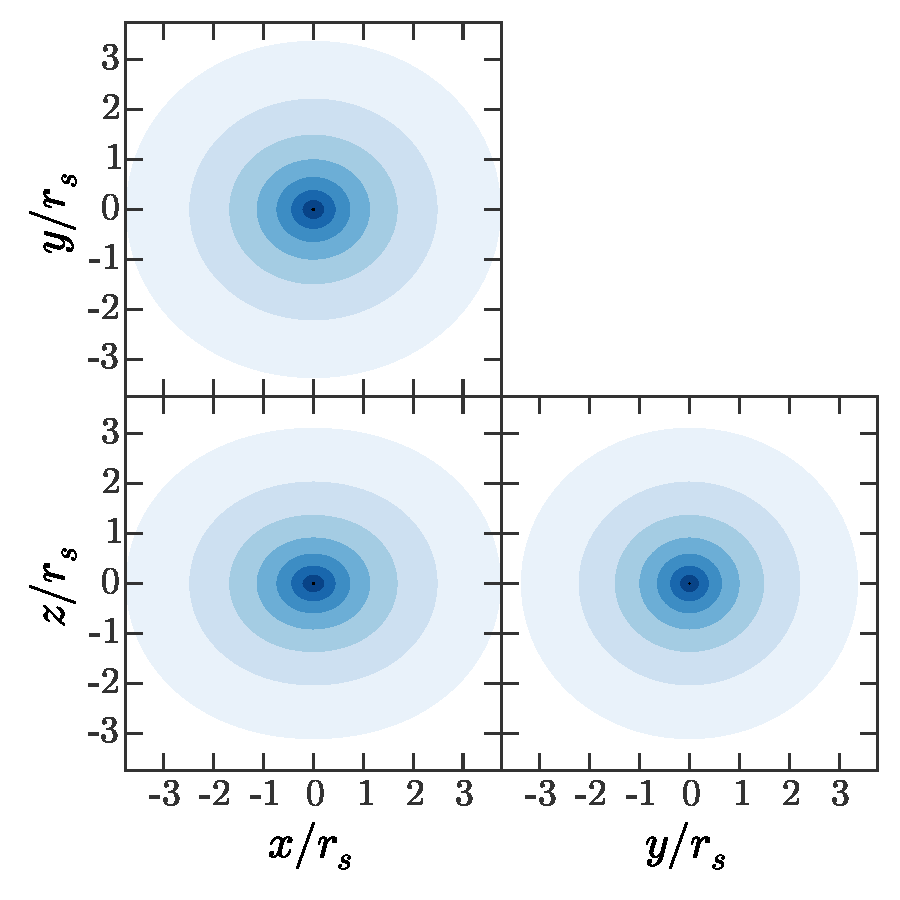
\includegraphics[width=0.75\textwidth]{figures/potential.pdf}
\caption{Rotation curve along $x$, $y$, and $z$ axes for the triaxial, NFW potential } \label{fig:potential}
\end{center}
\end{figure*}

This potential is a simple and unrealistic model for the total potential of a Milky-Way-like galaxy, however it represents a conservative choice for exploring the effect of chaos in the halos of such galaxies. Realistic Falactic potentials will have a significant component due to the disk and bulge and may have twisting inertia tensors (cite), radially changing axis ratios \citep[e.g.,][]{veraciro11}, significant substructure \citep{zemp09}, or time dependence (either from bulk rotation, mass growth, mergers, etc.; cite). We expect all of these effects to increase the amount and influence of chaos; see the Discussion (Section~\ref{sec:discussion}) for a few simple demonstrations.

\subsection{Orbit integration}\label{sec:integration}

We use the Dormand-Prince 8th-order Runge-Kutta scheme (TODO: cite Dormand 1981) to integrate orbits in the above potential. In particular, we use the Python wrapper to the FORTRAN routines provided in the Scipy package \citep{scipy}. For all orbits, we ensure that energy is conserved to $\Delta E/E_0 \leq 10^{-9}$ by the end of integration. Unless otherwise specified, orbits are integrated for $\sim$250 orbital periods with 500 steps per orbital period. Some box orbits require more internal integration steps in order to conserve energy to the required level. 

\subsection{Lyapunov exponents} \label{sec:lyap}

The simplest and perhaps most well-known method for assessing chaotic motion is to analyze the Lyapunov spectrum or maximum Lyapunov exponent (MLE) of an orbit. Defining the vector $\bs{w} = (q_1,...,q_N,p_1,...,p_N)$ for some set of canonical coordinates $(q_i,p_i)$, we can write Hamilton's equations as 
\begin{equation}
	\dot{\bs{w}} = \bs{\mathcal{J}} \frac{\partial H}{\partial \bs{w}} = f(\bs{w}) \label{eq:ham}
\end{equation}
where $\bs{\mathcal{J}}$ is the $2N \times 2N$ canonical Poisson tensor (also called the symplectic matrix) defined by
\begin{equation}
	\bs{\mathcal{J}} = \left( \begin{array}{c:c} 0 & \ident \\ \hdashline -\ident & 0 \end{array} \right)
\end{equation}
with $N$-dimensional identity matrices $\ident$. If we consider a nearby phase-space position, $\bs{w}'$, separated from $\bs{w}$ by an infinitesimal deviation, $\delta \bs{w}$, such that $\bs{w}' = \bs{w} + \delta \bs{w}$. We can expand to linear order in the deviation about the parent orbit and write the equations of motion for the deviation as follows
\begin{align}
	\dot{\bs{w}}' &= f(\bs{w}')\\
	\dot{\bs{w}} + \dot{\delta \bs{w}} &= f(\bs{w} +  \delta \bs{w})\\
	\dot{\bs{w}} + \dot{\delta \bs{w}} &\approx f(\bs{w}) + \jac_{\bs{w}}\cdot\delta \bs{w} + \mathcal{O}(\delta \bs{w}^2)\\
	\dot{\delta \bs{w}} &\approx \jac_{\bs{w}} \cdot  \delta \bs{w}\label{eq:deviate}
\end{align}
where $\jac$ is the Jacobian of Eq.~\ref{eq:ham}, evaluated at the parent orbit (the Hessian of the Hamiltonian). For chaotic orbits, the maximum eigenvalue of the solution matrix to Eq.~\ref{eq:deviate} is positive real, leading to exponential divergence of nearby orbits. 

Computing the Lyapunov spectrum for a given orbit is often not necessary if one is only interested in characterizing the degree of chaos. Instead, it is often more efficient to compute the maximum Lyapunov exponent by estimating the finite-time maximum Lyapunov exponent (FTMLE), defined as 
\begin{equation}
	l_{\rm max}(t) = \frac{1}{t}\ln \frac{\|\delta \bs{w}(t)\|}{\|\delta \bs{w}_0\|}.\label{eq:lmax}
\end{equation}
The maximum Lyapunov exponent is the limit as $t\rightarrow \infty$ of the FTMLE
\begin{equation}
	\lambda_{\rm max} = \lim_{t\rightarrow\infty}l_{\rm max}(t). \label{eq:lyapmax}
\end{equation}
Numerically computing this quantity is not trivial because (1) obviously the limit to infinity is not possible and (2) the norm of the deviation vector $\|\delta \bs{w}(t)\|$ is expected to increase exponentially for chaotic orbits, leading to numerical problems. To circumvent these issues, it is sufficient to instead start a nearby orbit with some small initial deviation with norm $\delta_0$, integrate for a sufficiently small amount of time, $\tau$, then renormalize the deviation back to the initial norm (e.g., cite Bennetin et al. 1976, Tabor 1989). 
%The following pseudocode outlines this procedure:\footnote{see Gary for Python implementation?}\\
%\begin{algorithmic}[1]
%\State {\bf define} orbital integration timestep, $h$, and number of steps, $K$
%\State {\bf define} initial norm of deviation vector, $\delta_0$, to be sufficiently small
%\State {\bf define} renormalization integration period, $\tau \ll hK$ 
%\For{each timestep when integrating the main orbit, $\bs{w}(t)$}
%\State step forward the orbit and deviation vector orbit by one timestep, $t_{i-1} \rightarrow t_i$
%\If {a normalization timestep}
%\State measure and store the length of the deviation vector, $\delta_i = \|\delta \bs{w}_i\|$
%\State renormalize the length of the deviation vector, $\delta \bs{w}_i = \delta \bs{w}_i (\delta_0/\delta_i)$
%\EndIf
%\EndFor 
%\end{algorithmic}
The FTMLE after a given number of timesteps, $N$, is then estimated as
\begin{equation}
	l_N = \frac{1}{N\tau}\sum_i^N \ln \, \delta_i
\end{equation}
where $\delta_i=\|\delta \bs{w}(t_i)\|$ and the MLE is
\begin{equation}
	\lambda_{\rm max} = \lim_{N\rightarrow \infty} l_N.
\end{equation}

For most regular orbits, deviations will grow close to linearly or as some power-law of time. 
%As we have seen (Section~\ref{sec:introduction}), if the orbit is regular, there exists a local transformation to action-angle variables where the angle variables increase linearly with time, $\theta_n \propto \Omega_n t$. We can look at small variations around the orbit defined by the above equations:\footnote{Note the implied summation in repeated indices in the above expression.}
%\begin{align}
%	\frac{d (\delta \theta_n)}{dt} &= \frac{\partial \Omega_n}{\partial J_m} \delta J_m
%\end{align}
%These equations are trivially integrated:
%\begin{align}
%	\delta \theta_n(t) &= \delta \theta_n(0) + \left(\frac{\partial \Omega_n}{\partial J_m} \delta J_m \right) t
%\end{align}
%It's clear then that the norm of the deviation vector grows linearly with time:
%\begin{align}
%	\|\delta \bs{w}(t)\| &= \left[\sum_n (\delta \theta_n(t))^2 + \sum_n (\delta J_n)^2\right]^{1/2}\\
%	&= \left[\sum_n \left(\delta \theta_n(0) + \frac{\partial \Omega_n}{\partial J_m} \delta J_m t\right)^2 + \sum_n (\delta J_n)^2\right]^{1/2}\\
%	&\propto t.
%\end{align}
From Eq.~\ref{eq:lmax} and Eq.~\ref{eq:lyapmax} it is evident that any deviation vector that grows as a power law with time, $t^k$, will asymptote to 0 from the limit 
\begin{equation}
	\lambda_{\rm max} \propto \lim_{t\rightarrow \infty} k \frac{\ln t}{t} = 0.
\end{equation}
At long times, the numerically computed MLE should approach 0 as $t^{-1}$ for regular orbits. For chaotic orbits, the divergence is exponential, and the limit should converge to the rate of the exponential: the Lyapunov exponent.

In practice, the MLE is often estimated as the mean of $l_N$ after the summation diverges from power-law behavior. Figure~\ref{fig:lyap-orbits} shows $l_N$ computed for two nearby orbits in the potential of Section~\ref{sec:potential}. In physical units and Cartesian coordinates, the initial conditions for the two orbits are:
\begin{align}
	\bs{x}_{0}^{(1)} &= (27.85, 0, 23.35)~{\rm kpc}\\
	\bs{v}_{0}^{(1)} &= (0, 115.37, 0)~{\rm km~s}^{-1}\\
	\bs{x}_{0}^{(2)} &= (27.85, 0, 23.10)~{\rm kpc}\\
	\bs{v}_{0}^{(2)} &= (0, 116.43, 0)~{\rm km~s}^{-1}.
\end{align}
Over-plotted on both panels are lines (dashed) that show $t^{-0.9}$ behavior. The MLE estimate continues towards zero for the regular orbit (top) but saturates for the chaotic orbit (bottom) and continues to increase at least until the end of our integration period. For mildly chaotic or ``sticky'' orbits, it can take integration periods of many hundreds or thousands of orbits to determine a reliable estimate of the Lyapunov exponent.

\begin{figure*}[!h]
\begin{center}
\includegraphics[width=0.75\textwidth]{figures/lyap-orbits.pdf}
\caption{ } \label{fig:lyap-orbits}
\end{center}
\end{figure*}

\subsection{Numerical estimation of fundamental frequencies}\label{sec:naff}

Bounded, regular orbits in a triaxial potential will have three fundamental frequencies, $\bs{\Omega}$, that determine the periodic behavior of motion (Eq.~\ref{eq:aafreq}). This implies that for any canonical coordinate, $q$, the motion in this coordinate can be decomposed as 
\begin{equation}
	q(t) = \sum^\infty_k a_k e^{i \omega_k t}
\end{equation}
where these frequencies, $\omega_k$, are linear, integer combinations of the fundamental frequencies
\begin{equation}
	\omega_k = \bs{n}_k \cdot \bs{\Omega}
\end{equation}
and the $a_k$ are complex amplitudes and $\bs{n}_k$ is an integer vector. \cite{laskar93} introduced a method for recovering the fundamental frequencies of an orbit that effectively uses a Hanning-filtered fast-Fourier transform (FFT) of complex combinations of the motion (e.g., $x(t) + i v_x(t)$). It has been shown that using a Hanning filter makes the accuracy in determining the frequencies scale as $\inttime^{-4}$ instead of $\inttime^{-1}$ for a standard FFT \citep{laskar99}, where $\inttime$ is the integration time. In each complex time series, once the frequency is found, the amplitude of the term is found by projecting back on to the function itself. The component is then subtracted from the time series, and this procedure continues iteratively until some breaking condition (for example, the amplitude of the next term is below some threshold). We follow \cite{valluri98} and refer to this method as ``Numerical Approximation of Fundamental Frequencies'' (NAFF) even though it differs slightly from the original method from Laskar.

If an orbit is chaotic, the motion can no longer be expressed in terms of a single set of fundamental frequencies because the actions and frequencies of the orbit change with time. For a weakly chaotic orbit, the orbit may act consistently periodic over long windows of time. NAFF will pick out a set of frequencies for such orbits that correspond to the largest peaks in the power spectrum of the stochastic orbits, however these peaks will change character with time. For more strongly chaotic orbits, the power spectrum will be quite noisy and the peak frequencies may change erratically when comparing two separate sections of orbit. The frequencies picked out by NAFF for such orbits will therefore represent the average periodic nature of the orbit over a given period, and these will vary dramatically if comparing two consecutive integration periods. Therefore, the frequency diffusion rate per orbit, $\fdrate$, is a good predictor for how chaotic an orbit is:
\begin{equation}
	\fdrate = \max_{\bs{a}}\,2(\bs{\Omega}_{T_1} - \bs{\Omega}_{T_2}) / \inttime \label{eq:fdrate}
\end{equation}
where $\bs{\Omega}_{T_1}$ and $\bs{\Omega}_{T_2}$ are the fundamental frequencies computed from two consecutive sections of orbit, $\inttime$ is the total integration time (over both sections), and the maximum is taken with relation to the corresponding amplitudes, $\bs{a}$, of the frequency components. The frequency diffusion rate as defined above (e.g., measured in the frequency with the largest amplitude) is better correlated with the strength of chaos in an orbit \citep{valluri??} but differs from the original definition of \cite{valluri98}.

NAFF has been applied to many problems in Solar System and Galactic dynamics, especially in the study of of orbits in triaxial systems. For more details about the method, see \cite{papaphilippou96, laskar, etc.}. We have implemented and tested our own implementation of NAFF in Python. This code is publicly available through the Gary package.\footnote{link to repo} Figure~\ref{fig:logfreqs} shows a test of the implementation in which we reproduce the frequency map at a fixed energy of an axisymmetric, logarithmic potential \cite[][pg. 260, Figure~3.45]{binneytremaine}. Plotted are the (Cartesian) frequency ratios recovered for a grid of iso-energy, box orbits integrated in the potential
\begin{equation}
	\Phi(x,y,z) = \frac{1}{2}\ln\left(x^2 + (y/0.9)^2 + (z/0.7)^2 + 0.1\right).
\end{equation}
In such a map, stable resonances appear as linear over-densities and unstable resonances appear as linear under-densities. 

\begin{figure*}[!h]
\begin{center}
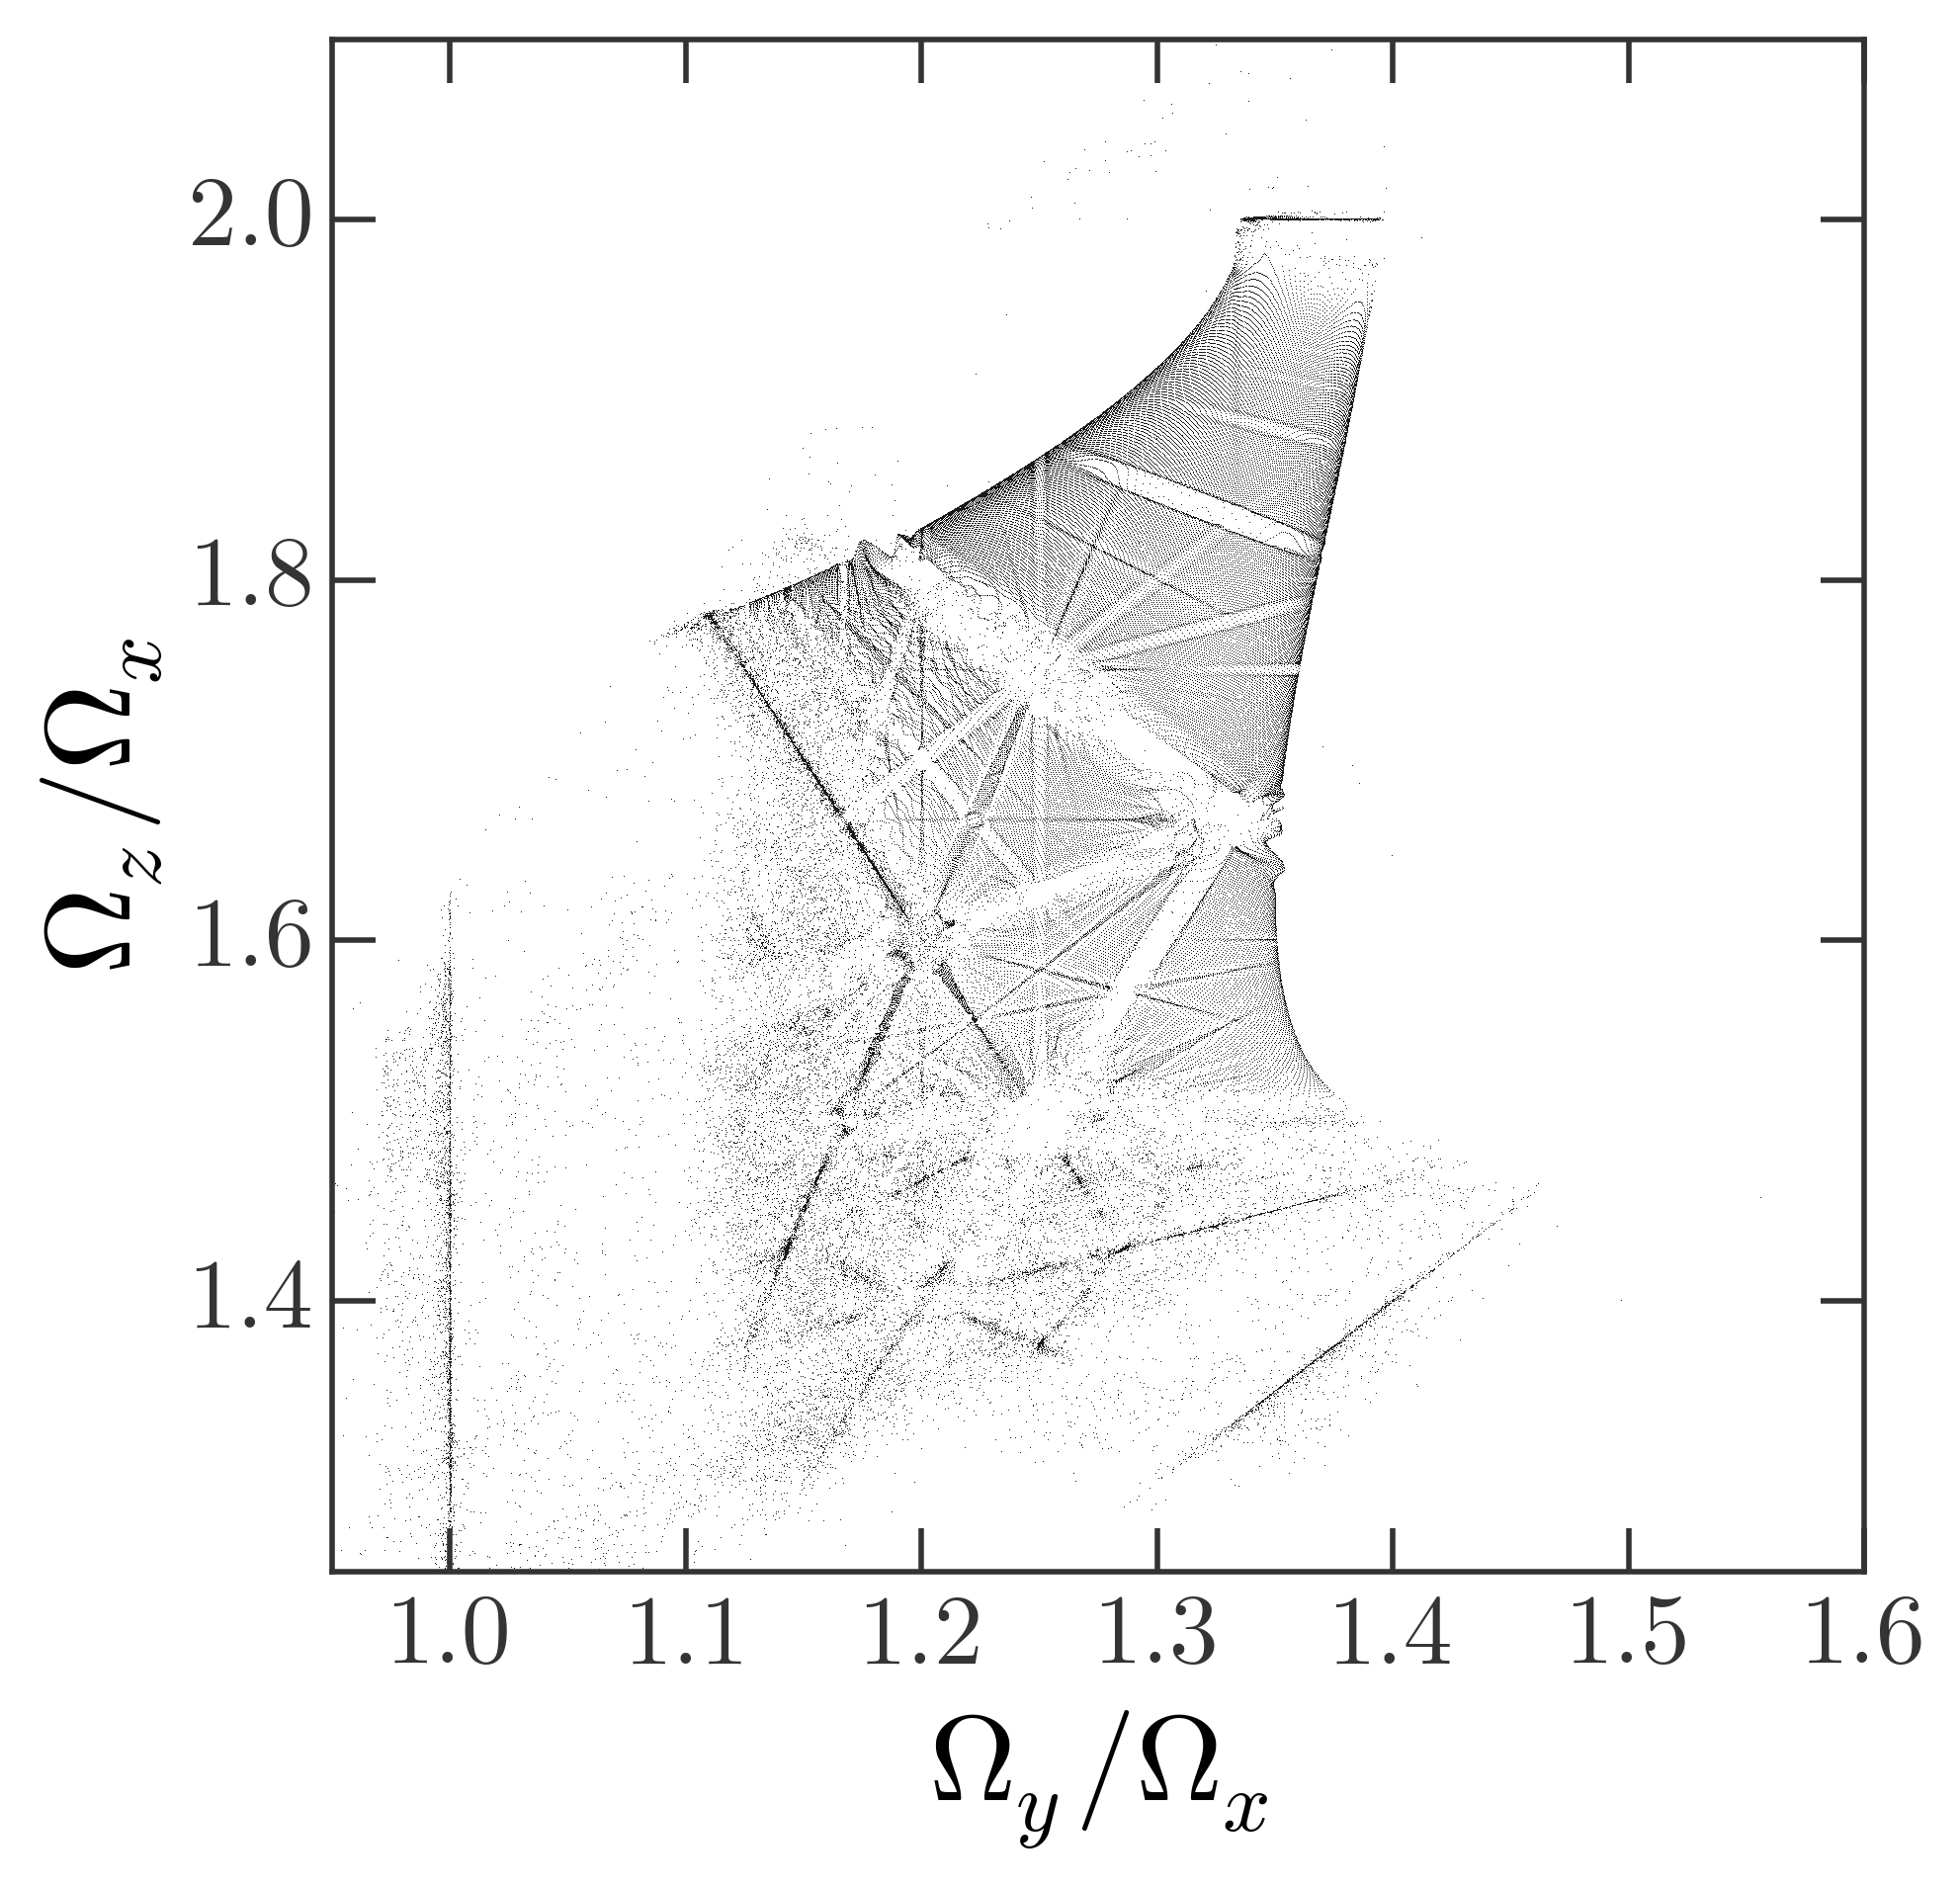
\includegraphics[width=0.75\textwidth]{figures/log-freqmap.png}
\caption{This is really just a placeholder that shows what I want to show here...} \label{fig:logfreqs}
\end{center}
\end{figure*}

We have found that for ``sticky'' or mildly chaotic orbits, reliably computing the Lyapunov exponent can require integration times equivalent to thousands of orbital periods. In comparison, owing to the precision of NAFF, detecting small frequency diffusion rates can be done with only hundreds of orbital periods. [example? comparison?] 
[Figure: for same orbits as in Lyapunov section, show frequency diffusion by computing frequencies in rolling windows?]

\subsection{Test particle ensembles} \label{sec:ensemble}

Our goal is to characterize the morphology of tidal debris along orbits generic to triaxial potentials. For example, it has been shown that along some chaotic orbits, tidal streams form large, diffuse ``fans'' of debris \citep[e.g.][]{pearson15, fardal14} [TODO: should I put sarahs paper here even though we didn't say this explicitly?], however, it is unknown how the resultant properties of the debris (e.g., density or length of the stream) depend on the degree of stochasticity. Further, quantifying the degree of stochasticity with, for example, the frequency diffusion rate represents a \emph{local} measure of chaos and it is unclear how this generalizes to the small but finite spreads in orbital characteristics common to debris that is tidally disrupted from globular clusters or dwarf satellite galaxies. To answer this question would require a massive exploration of parameter space -- both in potential and in orbits -- and thus would require a prohibitive number of N-body simulations to truly analyze the disruption process in all situations.

We therefore take a simplified approach and consider small ensembles of particles meant to represent debris disrupted from a single tidal disruption event of a low-mass progenitor. For a given set of orbital initial conditions -- the parent orbit -- we find the position of the nearest pericenter, initialize a small ensemble of test particle orbits around this position, then follow the orbits of all of these test particles for some evolution time, $T_{\rm ev}$. For a given mass scale, the ensemble particle position and velocity offsets are assumed to be Normal-distributed away from the parent orbit with spreads set by the tidal radius in position and velocity scale in velocity \citep[e.g.,][]{johnston98, apw14}. If $(\bs{x}_0,\bs{v}_0)$ are the parent orbit initial conditions at pericenter, then $(\delta\bs{x}_i,\delta\bs{v}_i)$ is the deviation vector of the $i$th particle and is drawn from
\begin{align}
	\delta\bs{x}_i &\sim \mathcal{N}(0, r_{\rm tide})\\
	\delta\bs{v}_i &\sim \mathcal{N}(0, \sigma_v)\\
	r_{\rm tide} &=|\bs{x}_0| \left(\frac{m}{3M_{\rm enc}(|\bs{x}_0|)}\right)^{1/3} \\
	\sigma_v &= |\bs{v}_0|\left(\frac{m}{3M_{\rm enc}(|\bs{x}_0|)}\right)^{1/3} 
\end{align}
where $M_{\rm enc}(r)$ is the mass enclosed of the host potential within radius $r$, and $m$ is the mass scale of the debris, and $|\cdot |$ is the Euclidean norm. For this work, we take $m=10^4~\msun$ to represent globular-cluster-like progenitors, and use the spherically-averaged enclosed mass to estimate the above scales.

As the particle ensembles evolve in time, we follow \citet[][hereafter MV96]{merritt96} and quantify the degree of mixing of the ensemble by computing the ``distance'' between the configuration space density of the ensemble at a given time, $\rho(\bs{x},t)$, with that of a distribution that is uniform over the energy hypersurface, $\rho_{E_0}(\bs{x})$, where $E_0$ is the energy of the parent orbit and thus hypersurface of interest. Our method differs in a few ways from that of MV96. First, MV96 use isoenergy ensembles of particles for following the density because that is the only way to guarantee that, if chaotic, nearly all orbits in the ensemble will lie on chaotic orbits. We instead use ensembles with small ($\approx$1\%) spreads in energy, but we still expect that such an ensemble around a parent chaotic orbit will reach a fully mixed state. The final distribution, rather than fill the energy hypersurface, will instead have some thickness around this surface. Around a typical regular orbit, each individual orbit will fill its torus ergodically -- that is, a surface with lower dimension than the energy hypersurface -- and thus, a small enough ensemble will never get ``close'' to the fully mixed state as defined above because it will remain confined into a subspace on the energy surface. In practice, only strongly chaotic systems will approach $\rho_{E_0}(\bs{x})$; the rate will depend on how stochastic the parent orbit is (e.g., as measured by the Lyapunov time or frequency diffusion rate), and also on how ``trapped'' the chaotic region is (a small chaotic region wedged between stable tori will take longer to appear chaotic, even if internally the frequency diffusion rate is large). However the difference in configuration space density between an ensemble undergoing chaotic mixing versus an ensemble around a regular orbit may be detectable over a much shorter timescale. The fully-mixed, normalized, configuration-space density that fills a given energy hypersurface, $E_0$, is 
\begin{align}
	\rho_{E_0}(\bs{x}) &= \int \dd^3v \, \rho_0 \, \delta(H - E_0)\\
	&= \int \dd^3v \, \rho_0 \, \delta\left(|\bs{v}|^2/2 + \Phi(\bs{x}) - E_0\right)\\
	&= 4\pi \int \dd v \, v^2 \, \rho_0 \, \delta\left(v^2/2 + \Phi(\bs{x}) - E_0\right)\\
	&= A \sqrt{E_0 - \Phi(\bs{x})}
\end{align}
where $A$ is a constant determined such that $\int \dd^3\bs{x} \, \rho_{E_0}(\bs{x}) = 1$, and $\delta(\cdot)$ is the Dirac delta function. 

Second, we compute the Kullback-Leibler divergence \citep[KL divergence;][]{kullback51} by estimating the configuration space density $\rho(\bs{x},t_j)$ using kernel density estimation (KDE)\footnote{We use an implementation from the Python package scikit-learn \citep{scikitlearn}.} with the ensemble of particle positions at time $t_j$, then use Monte Carlo integration to evaluate the KL divergence rather than evaluate the integral over a three dimensional grid. The KL divergence, $D_{\rm KL}$, is a measure of the relative Shannon entropy between two normalized density functions, $p(x)$ and $q(x)$,
\begin{equation}
	D_{\rm KL} = \int \dd x \, p(x) \ln \frac{p(x)}{q(x)}
\end{equation}
We would like to compute 
\begin{align}
	D_{\rm KL}(t_j) &= \int \dd^3 \bs{x} \, \rho(\bs{x},t_j) \ln \frac{\rho(\bs{x},t_j)}{\rho_{E_0}(\bs{x})}
\end{align}
however, we only have an estimate of the density $\rho_{\rm KDE}(\bs{x},t_j) \approx \rho(\bs{x},t_j)$. Using samples from this KDE estimated density, $\bs{x}_i$, the KL divergence is
\begin{align}
	D_{\rm KL}(t_j) &\approx \frac{1}{N} \sum_i^N \ln \frac{\rho_{\rm KDE}(\bs{x}_i,t_j)}{\rho_{E_0}(\bs{x}_i)}\\
	\bs{x}_i &\sim \rho_{\rm KDE}(\bs{x},t_j)\label{eq:sampled_from}
\end{align}
where Equation~\ref{eq:sampled_from} indicates that the $\bs{x}_i$ are samples from the KDE density. For any computation of the density estimate, we use 10-fold cross-validation to find the optimal kernel bandwidth, $\sigma_{\rm KDE}$, by maximizing the likelihood of withheld particles. Figure~\ref{fig:DKL} shows $D_{\rm KL}$ as a function of time for a regular (black) and chaotic (blue) orbit. The chaotic orbit ensemble mixes much faster than the regular orbit ensemble.

\begin{figure*}[!h]
\begin{center}
\includegraphics[width=0.75\textwidth]{figures/D_KL.pdf}
\caption{This is really just a placeholder that shows what I want to show here...} \label{fig:DKL}
\end{center}
\end{figure*}

\section{Experiments}\label{sec:experiments}

\subsection{Orbital properties: frequencies, frequency diffusion, and Lyapunov exponents}

We start by studying the properties of isoenergy orbits in the potential described above. We generate grids of initial condition along the $xz$ ($y=0$) and $yz$ ($x=0$) planes\footnote{Recall that $x$ is the major, $y$ the intermediate, and $z$ the minor axis.} all with the same energy, $E=XXX$. For the $xz$ orbits, we fix $v_x = v_z = 0$, and compute $v_y$ from the energy. Similarly, for the $yz$ orbits, we fix $v_y = v_z = 0$, and compute $v_x$ from the energy. We integrate the orbits as described in Section~\ref{sec:integration} and compute the fundamental frequencies of each orbit with NAFF. Figure~\ref{fig:freqmap} shows frequency maps for the $xz$ (left) and $yz$ (right) grids. For short-axis tubes, the frequencies plotted are the radial frequency, $\Omega_r$, the azimuthal frequency around the $z$ axis, $\Omega_\phi$, and the oscillation along the $z$ axis, $\Omega_z$. For long-axis tubes, the frequencies plotted are the radial frequency, $\Omega_r$, the azimuthal frequency around the $x$ axis, $\Omega_\phi$, and the oscillation along the $x$ axis, $\Omega_x$. Box orbits are not shown. Already evident in these panels is that many of the orbits are regular: the transformed, even-spaced sampling of the initial conditions is preserved in the frequency transformation, implying that the frequencies for many orbits do not change appreciably. Also apparent is resonant trapping,  which appear as over-dense, linear features in these frequency maps. 

The majority of the orbits generated on these grids are tube orbits, which preserve a sense of rotation about one of the principal axes of the potential and are generally centrophobic. Tube orbits are generally less stochastic than box orbits -- the other major class of orbits in triaxial potentials -- which tend to plunge deep into the inner regions of the potential. Thin tidal streams are thought to form along tube orbits rather than box orbits because of the fast disruption expected for stellar systems on radially plunging orbits. The major classes of stable tube orbits circulate about either the major or minor axis; the most prominent orbits are the short-axis and outer long-axis tubes, but these grids do generate some inner long-axis tubes and box orbits. Orbits that try to circulate about the intermediate axis tend to be highly irregular and do not preserve their sense of circulation for long periods of time. NAFF recovers fundamental frequencies for an orbit faster (with a fewer number of terms) when the coordinates used are ``close'' to the angle variables \cite[PL96][]{papaphilippou96}. PL96 show that a good choice of coordinates for tube orbits are the Poincar\'e symplectic polar coordinates, a set of canonical coordinates similar to cylindrical coordinates. For approximately XX\% of the orbits, NAFF fails to recover the frequencies (similar difficulties were reported in \cite{valluri98} and \cite{papaphilippou96} for recovering certain tube orbit frequencies).

\begin{figure}[h]
\centering
	\includegraphics[width=0.45\columnwidth] {figures/freqmap_xz.png}
	\includegraphics[width=0.45\columnwidth] {figures/freqmap_yz.png}
	\caption{Not the final figures. Need to re-make with same axis limits, remove labels, put in same PDF file...etc.} 
	\label{fig:freqmap}
\end{figure}

For each orbit, we also compute the frequency diffusion rate per orbit, $\fdrate$ (Equation~\ref{eq:fdrate}) by computing the frequencies for the first half and second half of the orbital time series separately. This rate is only a measure of the time-averaged diffusion rate because the frequencies are computed for long segments of orbit, but \cite{valluri??} [...]. Figure~\ref{fig:diffusionmap} shows maps of the frequency diffusion for the $xz$ (left) and $yz$ (right) grids: plotted are the initial conditions for all orbits colored by $\log_{10}(\fdrate)$ (white points are strongly chaotic, black are regular). The rich structure of unstable resonances apparent in these frequency diffusion maps highlight the accuracy of NAFF. It seems that tube orbits in these potentials are mostly regular or only mildly chaotic, however islands of stronger chaos do appear, especially at the intersections of unstable resonances. The bright, unstable regions in these maps are a visualization of the Arnold web at this energy. It is evident that these unstable regions are interconnected and therefore a tube orbit that starts, for example, in the lower left-hand region of one of these maps could  theoretically end up as a box orbit (along the zero-velocity curve) at some point in it its history (but the timescale for this to happen is likely prohibitively long). Figure~\ref{fig:diffusionrates} shows histograms of $\log_{10}(\fdrate)$ for all orbits in each initial condition grid for box and tube orbits separately. [...1-2 sentences discussion this (need to wait to see final figure)]

\begin{figure}[h]
\centering
	\includegraphics[width=0.45\columnwidth] {figures/diffusion_map_xz.png}
	\includegraphics[width=0.45\columnwidth] {figures/diffusion_map_yz.png}
	\caption{Not the final figures. Need to re-make with same axis limits, remove labels, put in same PDF file...etc.} 
	\label{fig:diffusionmap}
\end{figure}

\begin{figure}[h]
\centering
	\includegraphics[width=0.45\columnwidth] {figures/diffusion_rate_hist_xz.pdf}
	\includegraphics[width=0.45\columnwidth] {figures/diffusion_rate_hist_yz.pdf}
	\caption{Not the final figures. Need to re-make with same axis limits, remove labels, put in same PDF file...etc. Separate box from tube orbits.} 
	\label{fig:diffusionrates}
\end{figure}

\begin{figure}[!h]
\centering
	\includegraphics[width=0.4\columnwidth] {figures/lyap_map_xz.png}
	\includegraphics[width=0.4\columnwidth] {figures/lyap_map_yz.png}
	\caption{Not the final figures. Need to re-make with same axis limits, remove labels, put in same PDF file...etc.} 
	\label{fig:lyapmap}
\end{figure}

We also compute the Lyapunov exponents for all orbits in the grid by integrating their orbits for 250 orbital periods. Figure~\ref{fig:lyapmap} shows the initial condition grids again, but now the greyscale intensity corresponds to the logarithm of the Lyapunov time, $t_\lambda = \lambda_{\rm max}^{-1}$. These Lyapunov exponent maps show that, for a fixed integration time, only the most chaotic orbits are identified. NAFF is able to detect small differences in the frequencies and thus measure small diffusion rates with comparable integration times.

Figure~\ref{fig:xx} shows a sample of regular orbits from these two grids, plotted in projection. The left column are orbits from the $xz$ grid and the right column shows orbits from the $yz$ grid. Orbits near a resonance are labeled with the integer vector associated with the nearest resonance. Figures~\ref{fig:chaotic1} and \ref{fig:chaotic2} show two chaotic orbits, one with a large $\fdrate$ and one with a small $\fdrate$ (labeled in the figure titles). The figures show projections of the orbit in three consecutive sections of orbit with $\sim$50 periods shown per panel.

\begin{figure*}[!h]
\begin{center}
\includegraphics[width=\textwidth]{figures/chaotic_orbit1.png}
\caption{Just a placeholder figure that has a similar shape to what I will put here} \label{fig:chaotic1}
\end{center}
\end{figure*}

\begin{figure*}[!h]
\begin{center}
\includegraphics[width=\textwidth]{figures/chaotic_orbit2.png}
\caption{Just a placeholder figure that has a similar shape to what I will put here} \label{fig:chaotic2}
\end{center}
\end{figure*}

\subsection{Ensemble properties: mixing of debris}

We measure the state of mixing of the debris as described above: we compute the KL divergence between the configuration-space density of the ensemble and the configuration-space density expected if the ensemble particles were uniformly distributed over the parent orbit energy hypersurface. 

a:
This measure can be computed at any time -- [we show two different maps of this quantity: one after 10 Gyr, one after 15 orbits?]

b: 
From the KL divergence, we compute a mixing time by measuring the slope or power law index?

[Measure mixing time from KLD(t), plot freq. diffusion time vs. mixing time, show we can predict morphology from orbital properties of progenitor?]

\subsection{Observable consequences of mixing}

Only effectively looking at debris disrupted from a single pericenter -- debris near progenitor constantly repopulated as more and more stuff disrupts out

Streams should be shorter? How to test this? Length of stream in angle at isodensity contour?

\section{Discussion}\label{sec:discussion}

Recovering the potential of triaxial systems is not trivial. Danger of orbit fitting because chaotic orbits can reproduce morphologies of regular orbits.

\subsection{Potential}

Time dependence

Radial dependence of axis ratios

Why not disk + bulge? What do we expect when we add? See later section for test of this...

Real disk will be self-consistent with halo, so this isn't really a fair test, but still...

\acknowledgements
The authors wish to thank Sarah Pearson, Andreas K\"upper, David Hogg, David Merritt, and the \emph{Stream Team} for useful comments and discussion.
APW is supported by a National Science Foundation Graduate Research Fellowship under Grant No.\ 11-44155. 
This research made use of Astropy, a community-developed core \texttt{Python} package for Astronomy \citep{astropy13}.
This work additionally relied on Columbia University's \emph{Hotfoot} and \emph{Yeti} compute clusters, and we acknowledge the Columbia HPC support staff for assistance.

\bibliographystyle{apj}
\bibliography{refs}

\end{document}
